\documentclass[8pt]{beamer}

\usetheme[progressbar=frametitle]{metropolis}
\setbeamercolor{background canvas}{bg=white}

\usepackage{appendixnumberbeamer}

\usepackage{booktabs}
\usepackage[scale=2]{ccicons}

\usepackage{pgfplots}
\usepgfplotslibrary{dateplot}

\usepackage{xspace}
\newcommand{\themename}{\textbf{\textsc{metropolis}}\xspace}

\usepackage{lineno,hyperref}
\usepackage{amsmath}
\usepackage{mathtools}
\usepackage{amssymb}
\usepackage{xcolor}
\usepackage{pdfpages}
\usepackage{caption}
\usepackage{subcaption}
\usepackage{tikz}
\usepackage{csvsimple}
\usepackage{smartdiagram}
\usesmartdiagramlibrary{additions}
\usepackage[export]{adjustbox}
\usepackage[document]{ragged2e}

\usepackage{amsbsy}
\newcommand*{\claps}[1]{\hbox to 0pt{\hss#1\hss}}
\newcommand*{\mat}[1]{\boldsymbol{\mathrm{#1}}}
\newcommand*{\subdims}[3]{\clap{\raisebox{#1}[0pt][0pt]{$\scriptstyle(#2 \times #3)$}}}
\fboxrule=1pt

\usepackage{soul}
\newcommand{\mathcolorbox}[2]{\colorbox{#1}{$\displaystyle #2$}}

\title{Sensitivity analysis of a control-oriented model of supercritical extraction}
\subtitle{}
% \date{\today}
\date{05.06.2023}
\author{Oliwer Sliczniuk}
\institute{Aalto University, Finland}

\titlegraphic{\includegraphics[trim = 8.5cm 7cm 8.5cm 7cm,clip,width=2cm]{Figures/logo.png} }

\begin{document}
	
	\begin{frame}
		\titlepage 
	\end{frame}
	
%	\begin{frame}{Contents}
%		\begin{enumerate}
%			\item Introduction to the process
%			\item Process model and assumptions
%			\item Methodology - forward sensitivity analysis
%			\item Simulation results
%			\item Sensitivity analysis results
%		\end{enumerate}
%	\end{frame}

	\begin{frame}[fragile]{SFE}
		What are advantages of supercritical fluid extraction?
		\begin{itemize}
			\item $CO_2$ non-flammable and non-toxic
			\item properties of $CO_2$ can be 'tuned' with operating conditions
			\item the critical point of $CO_2$ is easily accessible 
			\item high selectivity
			\item easy separation of the solvent (if there is no co-solvent)
		\end{itemize}
	
		\begin{figure}[!h]
			\centering
			\includegraphics[trim = 2.5cm 8cm 18cm 7cm,clip,width=0.31\textwidth]{Figures/Compressibility.pdf}
			\includegraphics[trim = 2.5cm 8cm 18cm 7cm,clip,width=0.31\textwidth]{Figures/RHO.pdf}
			\includegraphics[trim = 2.5cm 8cm 18cm 7cm,clip,width=0.31\textwidth]{Figures/CP.pdf}
			\caption{Properties of $CO_2$}
			\label{fig:SFE_drawing}
		\end{figure} 
	
	\end{frame}
	
%	\begin{frame}[fragile]{$CO_2$ properties}
%		\begin{figure}[!h]
%			\centering
%			\includegraphics[trim = 2.5cm 8cm 2.5cm 7cm,clip,width=0.8\textwidth]{Figures/Compressibility.pdf}
%			\includegraphics[trim = 2.5cm 8cm 2.5cm 7cm,clip,width=0.8\textwidth]{Figures/RHO.pdf}
%			\includegraphics[trim = 2.5cm 8cm 2.5cm 7cm,clip,width=0.8\textwidth]{Figures/CP.pdf}
%			\caption{Properties of $CO_2$}
%			\label{fig:SFE_drawing}
%		\end{figure} 
%	\end{frame}

%	\section{Model description}
	
%	\begin{frame}[fragile]{SFE}
%		\begin{figure}[!h]
%			\centering
%			\includegraphics[trim = 5cm 0cm 5cm 0cm,clip,height=0.70\textheight]{Figures/SFE_Diagram.pdf}
%			\caption{Schematic representation of SFE process}
%		\end{figure} 
%	\end{frame}

	\begin{frame}[fragile]{SFE - assumptions}
		\begin{minipage}[b]{0.475\textwidth}
			\begin{figure}[!h]
				\centering
				\includegraphics[trim = 5cm 0cm 5cm 0cm,clip,width=\textwidth]{Figures/SFE_Diagram.pdf}
				\caption{Schematic representation of SFE process}
			\end{figure} 
		\end{minipage}
		\hfill \vrule \hfill
		\begin{minipage}[b]{0.475\textwidth}
			Assumptions:
			\begin{itemize}
				\item Quasi-one-dimensional model
				\item Negligible external diffusion
				\item Low-Mach number assumption
				\item No pressure drop
				\item Pseudo-single component
				\item Negligible thermal properties of solid phase
				\item Uniform distribution of the particles
				\item Varying void fraction along the extractor
			\end{itemize}
	\end{minipage}
	\end{frame}
	
	\begin{frame}{Model of an extractor}
		
		{\tiny\begin{align*}
		\intertext{(1) Fluid phase mass balance [1]}
				&\frac{\partial {\color{blue}c_f}(t,z)}{\partial t}
				+ \underbrace{\frac{1}{{\color{magenta}\phi}} \frac{\partial \left( {\color{blue}c_f}(t,z) u\right)}{\partial {\color{blue}z}}}_{Convection}
				= \underbrace{\frac{1-{\color{magenta}\phi}}{{\color{magenta}\phi}} {\color{blue}r_e}(t,z) }_{Kinetic}
				+ \underbrace{\frac{1}{{\color{magenta}\phi}} \frac{\partial}{\partial {\color{blue}z}} \left( \mathcolorbox{yellow}{D^M_e} \frac{\partial {\color{blue}c_f}(t,z)}{\partial {\color{blue}z}} \right) }_{Diffusion}
				\\
				%		\end{align*}}
		\intertext{(2) Solid phase mass balance [1]}
		%		{\scriptsize\begin{align*}
				&\cfrac{\partial \textcolor{blue}{c_s}(t,z)}{\partial t} = - \underbrace{{\color{blue}r_e}(t,z)}_{Kinetic}\\
				%		\end{align*}}
		\intertext{(3) Heat balance [2]}
		%		{\scriptsize\begin{align*}
				&\cfrac{\partial \left({\color{orange}\rho_f}({\color{blue}T}(t,z),{\color{red}P}(t)) {\color{blue}h}(t,z) A_f\right)}{\partial t} - \cfrac{\partial \left({\color{red}P}(t) A_f\right)}{\partial t} = 
				\underbrace{- \cfrac{\partial \left( {\color{orange}\rho_f}({\color{blue}T}(t,z),{\color{blue}P}(t)) {\color{blue}h}(t,z) A_f v \right)}{\partial {\color{blue}z}} }_{Convection}
				+ \underbrace{\cfrac{\partial}{\partial {\color{blue}z}} \left( k \cfrac{\partial {\color{blue}T}(t,z)}{\partial {\color{blue}z}} \right)}_{Diffusion}\\
%		\intertext{(4) Pressure}
%				&\cfrac{\partial \textcolor{blue}{P}(t)}{\partial t} = \cfrac{P(t)-P(t-1)}{\partial t}\\
%
				\\ \hline
		\intertext{Extraction kinetic [1]}
				{\color{blue}r_e}(t,z) &= -\cfrac{ \mathcolorbox{yellow}{D_i} } {{\color{magenta} \mu l^2} }\left({\color{blue}c_s}(t,z) \mathcolorbox{yellow}{k_m}  - {\color{blue}c_f}(t,z) \right)
		\intertext{Output function [3]}
		%		{\scriptsize\begin{align*}
				\textcolor{blue}{y}(t) &= \textcolor{blue}{g}(x(t)) = \int_{0}^{t_f} \textcolor{red}{Q}(t)  \textcolor{blue}{c_f}(t,z) |_{z = L} dt =
				\int_{0}^{t_f} \textcolor{red}{u}(t)  \textcolor{green}{A} \textcolor{blue}{c_f}(t,z) |_{z = L} dt =
				\iff \cfrac{ \partial \textcolor{blue}{y}(t)}{\partial t} = \textcolor{red}{u}(t) A \textcolor{blue}{c_f}(t,z) |_{z = L}\\
	 	\intertext{Equation of state - Peng-Robinson}
		%		{\scriptsize\begin{align*}
				 \textcolor{orange}{P} & \left( \textcolor{blue}{T}(t,z), \textcolor{blue}{\rho}(t,z) \right) = \frac{R \textcolor{blue}{T}(t,z) }{\textcolor{blue}{v}(t,z)-b} - \frac{a}{\textcolor{blue}{v}(t,z)(\textcolor{blue}{v}(t,z)+b)+b(\textcolor{blue}{v}(t,z)-b)}; \quad \textcolor{blue}{v}(t,z) = \cfrac{1}{ \textcolor{blue}{\rho}(t,z) }
		\end{align*}}
	\hrule
	\Tiny{[1] E. Reverchon, Mathematical modeling of supercritical extraction of sage oil, AIChE J 42 (6), 1996}\\
	\Tiny{[2] John D. Anderson. Computational fluid dynamics the basic with applications. McGraw-Hill, 1995}\\
	\Tiny{[3] H. Sovova, R. Komers, J. Kucuera, and J. Jezu. Supercritical carbon dioxide extraction of caraway essential oil. Chemical Engineering Science, 1994}
	\end{frame}

	\begin{frame}[fragile]{Model discretization}
		\footnotesize{
			\begin{align*}
				\cfrac{d x(t)}{d t} &= 
				\begin{bmatrix}
					\cfrac{d c_{f_1}(t)}{d t}   	\\
					\vdots					   		\\
					\cfrac{d c_{f_{N_z}}(t)}{d t} 	\\
					\cfrac{d c_{s_1}(t)}{d t}   	\\
					\vdots					   		\\
					\cfrac{d c_{s_{N_z}}(t)}{d t}	\\
					\cfrac{d h_1(t)}{d t} 	   		\\
					\vdots 					   		\\
					\cfrac{d h_{N_z}(t)}{d t} 		\\
					\cfrac{d P(t)}{dt}				\\
					\cfrac{d y(t)}{dt}
				\end{bmatrix}
				=
				\begin{bmatrix}
					F_1 \left(c_f(t),c_s(t),T(t), y(t); \Theta \right)\\ 
					\vdots\\ 
					F_{N_z} \left(c_f(t),c_s(t),T(t), y(t); \Theta \right)\\ \\
					F_{N_z+1} \left(c_f(t),c_s(t),T(t), y(t); \Theta \right)\\
					\vdots\\
					F_{2N_z} \left(c_f(t),c_s(t),T(t), y(t); \Theta \right)\\ \\
					F_{2N_z+1} \left(c_f(t),c_s(t),T(t), y(t); \Theta \right) \\
					\vdots\\
					F_{3N_z} \left(c_f(t),c_s(t),T(t), y(t); \Theta \right) \\ \\
					F_{3N_z+1} \left(c_f(t),c_s(t),T(t), y(t); \Theta \right) \\ \\
					F_{3N_z+2} \left(c_f(t),c_s(t),T(t), y(t); \Theta \right) 
				\end{bmatrix}
				= F \left( t; \Theta \right)
		\end{align*} }\\
		where $x \in \mathbb{R}^{N_x = 3N_z+2} $ and $\Theta \in \mathbb{R}^{N_\Theta =  N_{\theta} + N_u } $
	\end{frame}

	
%	\begin{frame}[fragile]{Parameter estimation}
%		\small{
%			Maximum likelihood estimation [4] is used to define the objective function of the parameter estimation problem
%			
%			{\footnotesize
%				\begin{equation}
%					\ln L = -\cfrac{n}{2} \left( \ln \sqrt{2 \pi} + \ln \mathcolorbox{yellow}{\sigma^2} \right)
%					- \cfrac{ \sum_{i=1}^{n} \left[  Y(t_i) - y(\theta , t_i) \right]^2 }{2 \mathcolorbox{yellow}{\sigma^2}}
%				\end{equation}
%			}
%			
%			The parameter estimation problem can be formulated as follow:
%			
%			{\footnotesize
%				\begin{equation*}
%					\begin{aligned} \label{EQ: Optimization_formulation_MLE}
%						&\hat{\theta}_{MLE} &= \arg \max_{\sigma, \theta \in \Theta} \ln L = \arg \max_{\sigma,\theta \in \Theta} p(\theta|y) \\
%						&\text{subject to}
%						& \dot{x} = f(t,x,\theta) \\
%						&& \dot{\theta} = 0 \\
%						&& \theta^{lb} \leq \theta \leq \theta^{ub}
%					\end{aligned}
%			\end{equation*} }
%			
%			If the measurement is 'cumulative', then each new observation includes the error of the previous observations, but the differences in measurement from one period to the next are independent. In such a case, the measurement data should be redefined as:
%			
%			{\footnotesize
%				\begin{align*}
%					Y(t_i) = \sum_{j=1}^{i} \left( Y(t_j) - Y(t_{j-1}) \right) = \sum_{j=1}^{i} \left( y(\theta, t_j) - y(\theta, t_{j-1}) \right) + \sum_{j=1}^{i} \epsilon_j 
%			\end{align*} }
%			
%			in which $\epsilon_j$ are independent random variables with $\mathbb{E}\{\epsilon_j\}$ and Var$\{\epsilon_i\} = \sigma^2$, a constant. 
%		}
%	
%		\hrule
%		\Tiny{[4] David Mautner Himmelblau. Process analysis by statistical methods, 1970.}
%	\end{frame}
	
	\begin{frame}[fragile]{Results of the simulation}
		\begin{figure}[!h]
			\centering
			\begin{subfigure}[b]{0.49\textwidth}
				\centering
				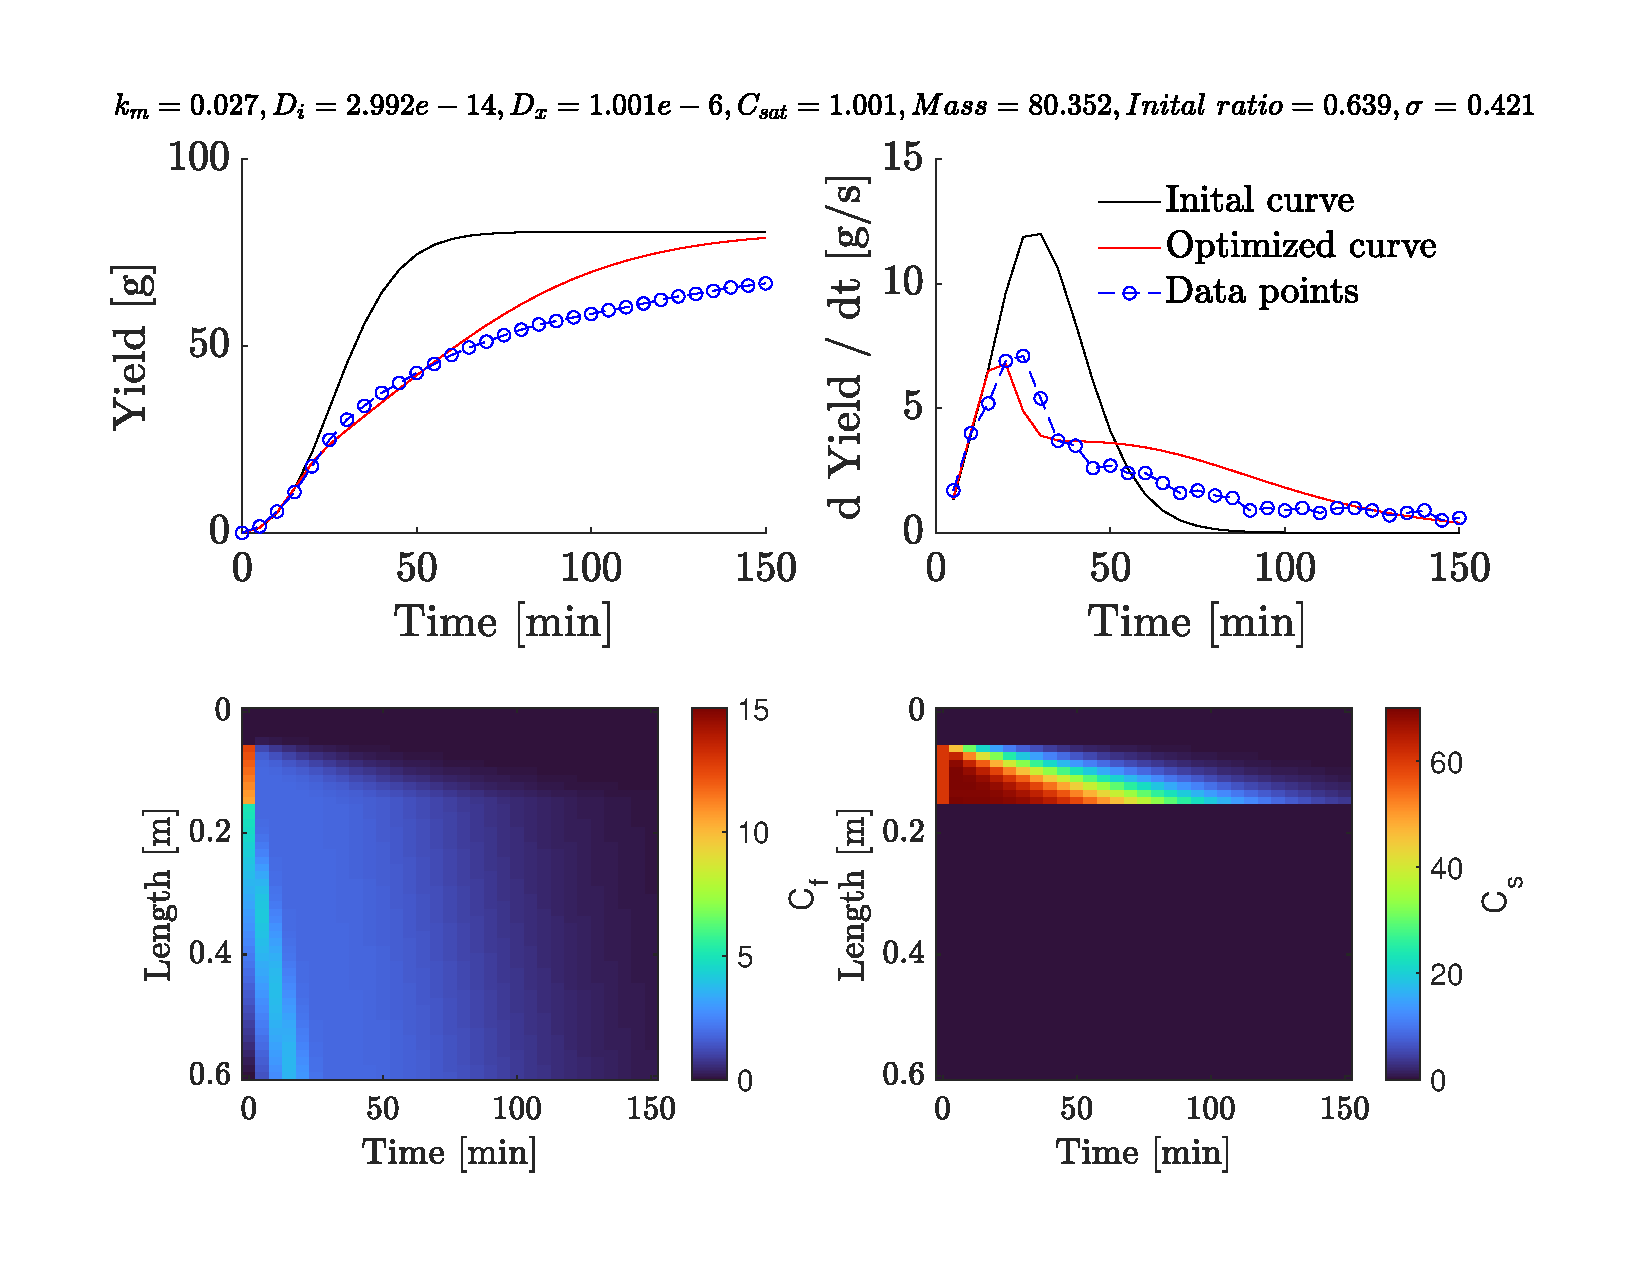
\includegraphics[trim = 2cm 10.5cm 2.5cm 2.02cm,clip,width=\textwidth]{Figures/Fitting_LUKE_T40_P200.pdf}
				\caption{Experiment at $40^\circ C$ and $200$ bar}
			\end{subfigure}
			\hfill
			\begin{subfigure}[b]{0.49\textwidth}
				\centering
				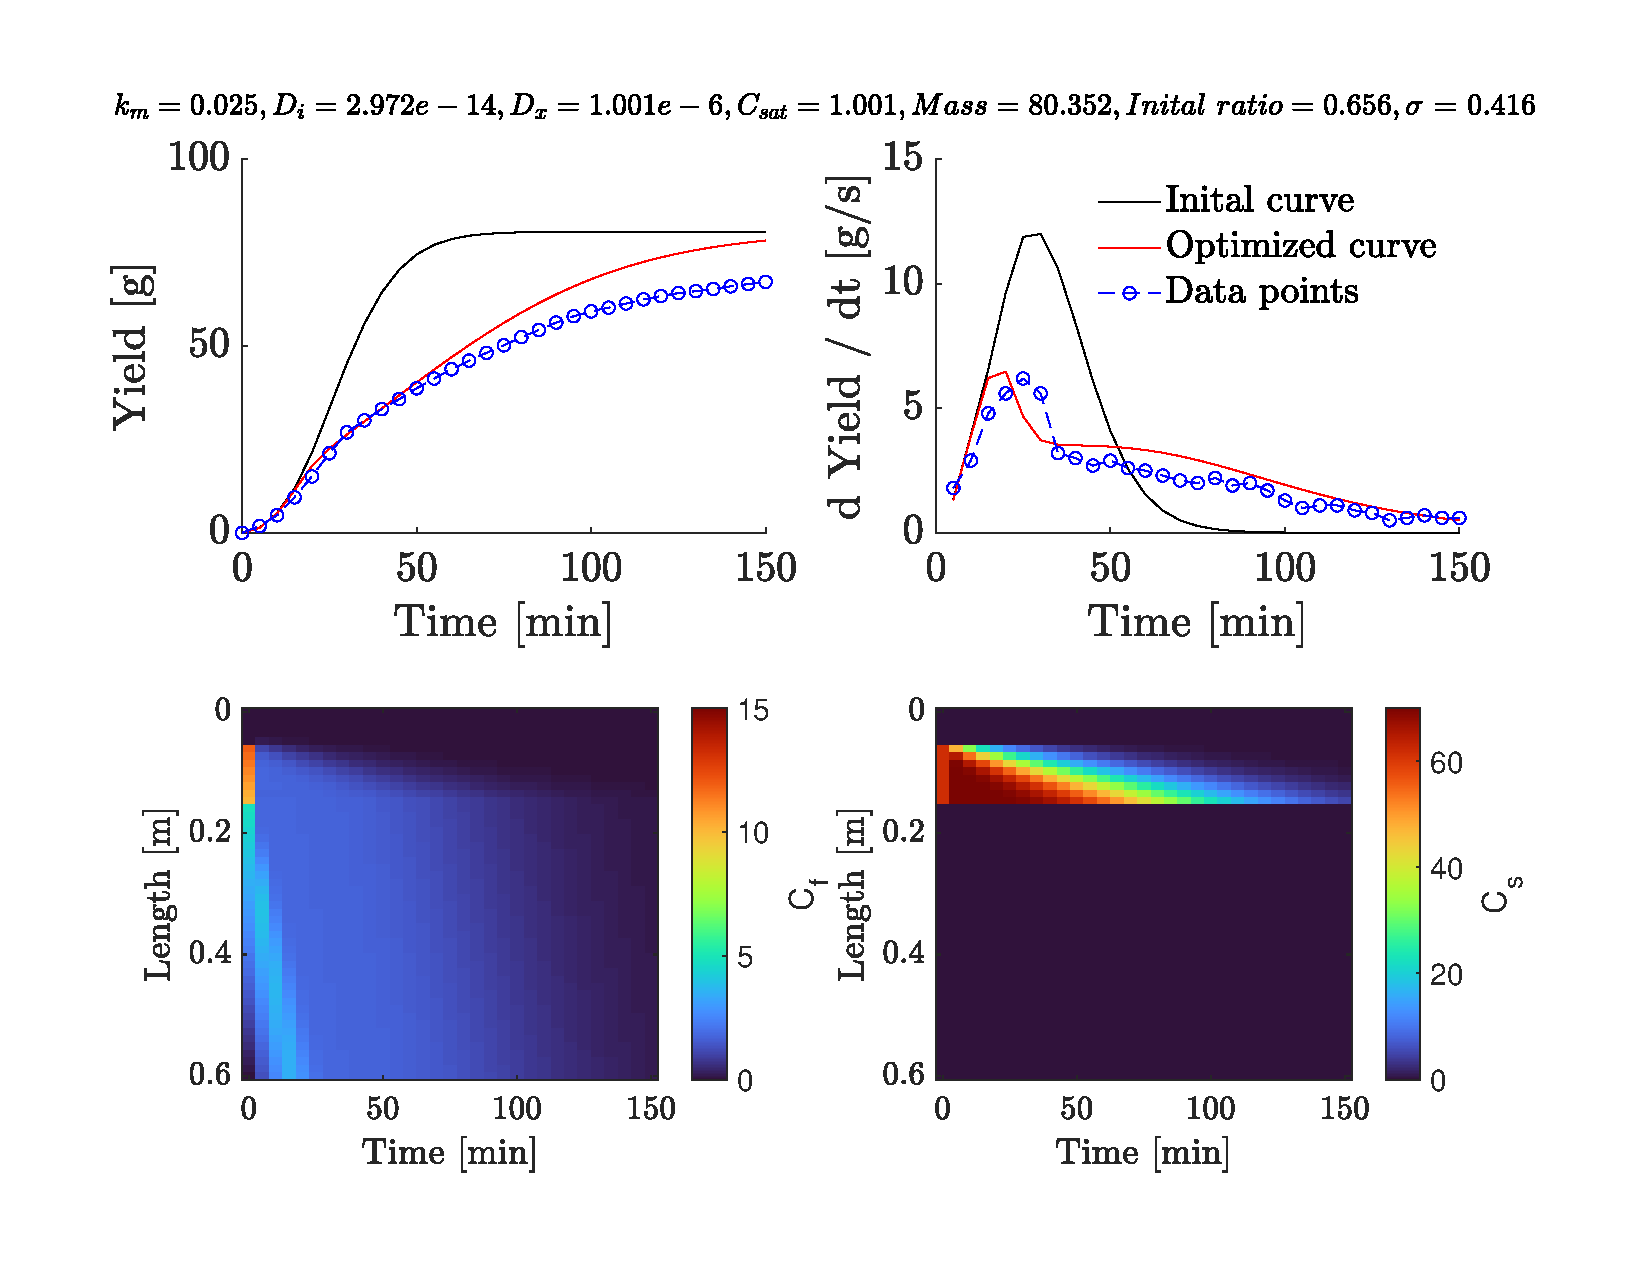
\includegraphics[trim = 2cm 10.5cm 2.5cm 2.02cm,clip,width=\textwidth]{Figures/Fitting_LUKE_T50_P200.pdf}
				\caption{Experiment at $50^\circ C$ and $200$ bar}
			\end{subfigure}
			\begin{subfigure}[b]{0.49\textwidth}
				\centering
				\includegraphics[trim = 2cm 10.5cm 2.5cm 2.02cm,clip,width=\textwidth]{Figures/Fitting_LUKE_T40_P300_org.pdf}
				\caption{Experiment at $40^\circ C$ and $300$ bar}
			\end{subfigure}
			\hfill
			\begin{subfigure}[b]{0.49\textwidth}
				\centering
				\includegraphics[trim = 2cm 10.5cm 2.5cm 2.02cm,clip,width=\textwidth]{Figures/Fitting_LUKE_T50_P300_org.pdf}
				\caption{Experiment at $50^\circ C$ and $300$ bar}
			\end{subfigure}
%			\begin{subfigure}[b]{0.60\textwidth}
%				\hspace*{-1.2cm}
%				\centering
%				\includegraphics[trim = 3cm 14cm 2.3cm 1cm,clip,width=\textwidth]{Figures/Trend_Lines_order_2.pdf}
%				\caption{Second-order polynomial regression of fitted parameters ($k_m$, $D_i$ and $D_e^M$) as a function of fluid density $\rho_f$}
%			\end{subfigure}
%			\hfill
%			\begin{subfigure}[b]{0.39\textwidth}
%				\begin{minipage}[t]{\textwidth}
%						\vspace*{-1.2cm}
%						\centering
%						\adjustbox{max width=\columnwidth}{%
%							\csvautobooktabular{Figures/estimation.csv} }
%				\end{minipage}
%				\caption{Parameter estimation results rounded to fifth decimal place}
%			\end{subfigure}
		\end{figure}
	\end{frame}
	
%	\section{Sensitivity Analysis}
	
	\begin{frame}[fragile]{Sensitivity Analysis}
		Local derivative-based methods involve taking the partial derivative of the output with respect to an input parameter. In sensitivity analysis the original system of equations is solved simultaneously with $\frac{\partial \textcolor{blue}{F}(x(t);\Theta)}{\partial \Theta}$, where $\Theta$ is a vector of all the parameters and the control variables.
		
		\small{
			\begin{align*}
				Z &= \cfrac{\partial x(t,\Theta)}{\partial \Theta} \nonumber \\
				\dot{Z}  &= \cfrac{\partial Z(t,\Theta)}{\partial t} = \cfrac{\partial }{\partial t} \left( \cfrac{\partial x(t,\Theta)}{\partial \Theta} \right) = \cfrac{\partial }{\partial \Theta} \left( \cfrac{\partial x(t,\Theta)}{\partial t} \right) = \cfrac{d F(x(t);\Theta)}{d \Theta} \\
				\cfrac{d F(x(t);\Theta)}{d \Theta} &=  \cfrac{\partial F(x(t);\Theta)}{\partial x(t)} \cfrac{\partial x(t)}{\partial \Theta} + \cfrac{\partial F(x(t);\Theta)}{\partial \Theta}  \\
				& = J_x(x(t);\Theta)S(x(t);\Theta) + J_\Theta(x(t);\Theta)
			\end{align*}
			%		}
		%		\tiny{
			%		\[
			%		\framebox[1.2cm]{\claps{\raisebox{0pt}[1.0cm][1.0cm]{$\mat {\cfrac{d F(x(t);\Theta)}{dp}} $}}\subdims{-1.5cm} {N_x} {N_p}} =
			%		\framebox[2.0cm]{\claps{\raisebox{0pt}[1.0cm][1.0cm]{$\mat J_x$}}\subdims{-1.5cm} {N_x} {N_x}} \ 
			%		\framebox[1.2cm]{\claps{\raisebox{0pt}[1.0cm][1.0cm]{$\mat S$}}  \subdims{-1.5cm} {N_x} {N_p}} + 
			%		\framebox[1.2cm]{\claps{\raisebox{0pt}[1.0cm][1.0cm]{$\mat J_p$}}\subdims{-1.5cm} {N_x} {N_p}}
			%		\]}
	}
	\tiny{
		\[
		\framebox[1.2cm]{\claps{\raisebox{0pt}[1.0cm][1.0cm]{$ {\cfrac{d F(x(t);\Theta)}{d\Theta}} $}}\subdims{-1.5cm} {N_x} {N_\Theta}} =
		\framebox[2.0cm]{\claps{\raisebox{0pt}[1.0cm][1.0cm]{$ {\cfrac{\partial F(x(t);\Theta)}{\partial x(t)}} $} }\subdims{-1.5cm} {N_x} {N_x}} \ 
		\framebox[1.2cm]{\claps{\raisebox{0pt}[1.0cm][1.0cm]{$ {\cfrac{\partial x(t)}{\partial \Theta}}$}}  \subdims{-1.5cm} {N_x} {N_\Theta}} + 
		\framebox[1.2cm]{\claps{\raisebox{0pt}[1.0cm][1.0cm]{$ {\cfrac{\partial F(x(t);\Theta)}{\partial \Theta}}$}}\subdims{-1.5cm} {N_x} {N_\Theta}}
		\]}
	
	\vspace*{0.5cm}
	\hrule
	\Tiny{[4] T. Maly, L. R. Petzold, Numerical methods and software for sensitivity analysis of differential-algebraic systems, Applied Numerical Mathematics 20 (1-2), 1996 }
	
	\end{frame}
	
	\begin{frame}[fragile]{Results of the sensitivity analysis - Internal diffusion}
		\begin{figure}[h]
			\centering
			\includegraphics[trim = 2cm 2cm 2cm 1cm,clip,width=0.9\textwidth,center]{Figures/D_iT50P200.pdf}	
			\caption{$50^\circ C,~200~bar$}
		\end{figure}
	\end{frame}
%	
%	\begin{frame}[fragile]{Results of the sensitivity analysis - Partition factor}
%		\begin{figure}[h]
%			\centering
%			\includegraphics[trim = 2cm 2cm 2cm 2cm,clip,width=0.9\textwidth,center]{Figures/k_m_all_long.pdf}	
%			\caption{$40-50^\circ C,~200-300~bar$}
%		\end{figure}
%	\end{frame}
	
	\begin{frame}[fragile]{Results of the sensitivity analysis - Flow-rate}
		\begin{figure}[h]
			\centering
			\includegraphics[trim = 2cm 2cm 2cm 1cm,clip,width=0.9\textwidth,center]{Figures/FT50P200.pdf}	
			\caption{$50^\circ C,~200~bar$}
		\end{figure}
	\end{frame}

	\begin{frame}[fragile]{Results of the sensitivity analysis - Flow-rate}
		\begin{figure}[h]
			\centering
			\includegraphics[trim = 2cm 2cm 2cm 2cm,clip,width=0.9\textwidth,center]{Figures/F_all.pdf}	
			\caption{$40-50^\circ C,~200-300~bar$}
		\end{figure}
	\end{frame}


	\begin{frame}[fragile]{Conclusion}
		The forward sensitivity analysis allows to 
		\begin{itemize}
			\item better understanding of the analysed model
			\item evaluated an influence of controls and parameters 
			\item identify sensitive and none-sensitive parameters
			\item spot modelling errors 
		\end{itemize}
		
	\end{frame}

		
\end{document}
